\documentclass[12pt,a4paper,oneside]{article}

\usepackage[pdftex,
            pdfauthor={Albert Zak},
            pdftitle={Design, Implementation and Evaluation of a Hands-off Build Pipeline for Erlang/OTP Projects},
            pdfsubject={Bachelor's Thesis},
            hidelinks,
            driverfallback=hypertex]{hyperref}
\usepackage[utf8]{inputenc}
\usepackage[T1]{fontenc}
\usepackage{geometry}
\usepackage{bookmark}
\usepackage{listings}
\usepackage[inline]{enumitem}
\usepackage{subcaption}
\usepackage{tabularx}
\usepackage{hhline}
\usepackage{algpseudocode}
\usepackage{tikz}
\usetikzlibrary{trees,arrows,fit,positioning,shapes.geometric}
\PassOptionsToPackage{usenames,dvipsnames,svgnames,table}{xcolor}
\usepackage{xcolor-solarized}
\usepackage{gitdags}
\usepackage[singlespacing]{setspace}
\usepackage[acronym,nopostdot,style=super,nonumberlist,nogroupskip]{glossaries}
\usepackage{fancyhdr}

\pagestyle{fancy}
\fancyhf{}
\cfoot{\thepage}
\renewcommand{\headrulewidth}{0pt}

\makeglossaries{}
\newacronym{mfa}{MF[A]}{Module, Function, and List of Arguments}
\newacronym{bif}{BIF}{Built-in Function}
\newacronym{erts}{ERTS}{Erlang Run-Time System}
\newacronym{vm}{VM}{Virtual Machine}
\newacronym{otp}{OTP}{Open Telecom Platform}
\newacronym{sasl}{SASL}{System Architecture Support Libraries}
\newacronym{os}{OS}{Operating System}
\newacronym{vcs}{VCS}{Version Control System}
\newacronym{api}{API}{Application Programming Interface}
\newacronym{ci}{CI}{Continuous Integration}
\newacronym{cli}{CLI}{Command Line Interface}
\newacronym{ram}{RAM}{Random Access Memory}
\newacronym{dsu}{DSU}{Dynamic Software Updating}
\newacronym{tls}{TLS}{Transport Layer Security}
\newacronym{http}{HTTP}{Hypertext Transfer Protocol}
\newacronym{lxc}{LXC}{Linux Containers}
\newacronym{aws}{AWS}{Amazon Web Services}
\newacronym{beam}{BEAM}{Bogdan/Björn's Erlang Abstract Machine}
\newacronym{ecs}{ECS}{Elastic Compute Cloud Container Service}
\newacronym{cow}{CoW}{Copy-on-Write}
\newacronym{appup}{appup}{Application Upgrade Instructions}
\newacronym{relup}{relup}{Release Upgrade Instructions}


\lstset{
  language=erlang,
  numbers=left,
  numberstyle=\small\color{lightgray},
  basicstyle=\ttfamily,
  frame=tb
}

\pdfpageheight=297mm
\pdfpagewidth=210mm
\geometry{a4paper, left=30mm, right=25mm, top=30mm, bottom=30mm}

\begin{document}

\cleardoublepage{}

\section*{Abstract}

The Erlang/OTP release process requires manual interaction at many steps. Previous work on automating Erlang/OTP Release generation has addressed parts of the process by abstracting the low-level mechanics of the build step, but tasks such as versioning and handling artifacts were left to the developer. This thesis presents a release generation tool designed for hands-off operation as part of a Continuous Integration pipeline. Tight coupling with Git allows reliable identification of releases by discarding numeric versions in favor of commit hashes, and a centralized release store takes care of handling artifacts. Evaluation of a reference implementation on six hosted Continuous Integration providers (\emph{CircleCI, Codeship, Semaphore, Shippable, Travis CI,} and \emph{Wercker}) demonstrates comparable run time and ease of setup.


\tableofcontents{}

\renewcommand{\glsnamefont}[1]{\textbf{#1}}
\doublespacing
\printglossary[nonumberlist,type=\acronymtype]
\singlespacing

\chapter{Introduction}

% Structure borrowed from Andrej Karpathy
% http://karpathy.github.io/2016/09/07/phd/

% 1 - X (+define X if not obvious) is an important problem

Continuous Deployment of software is an important problem.
Erlang/OTP Releases has first-class support for zero-downtime hot code upgrades.

% 2 - The core challenges are this and that.

The Erlang/OTP release and deployment process requires manual interaction at many steps.
A developer needs to touch various configuration files to edit version numbers.
Existing build tools produce upgrade scripts that sometimes need manual tweaking, such as rearranging instructions because of dependency issues.
Moreover, builds created on developer's machines are not deterministic. Tooling expects previously built releases to exist in specific directories on the local file system.
Deployment is a manual multi-step process. Current best practices advocate the use of \lstinline{scp} to copy the built release to the production machines. Then one has to attach an Erlang shell to the running node and issue various commands to actually perform the upgrade. This is not an appropriate process for a modern Continuous Delivery pipeline.

% 3 - Previous work on X has addressed these with Y, but the problems with this are Z.

Previous work on automating Erlang/OTP Release generation has addressed parts of the process by abstracting the low-level mechanics of the build step, but tasks such as versioning, release management, and deployment were left to the developer.

% 4 - In this work we do W.

This thesis proposes an integrated pipeline for building and deploying Erlang/OTP projects, including: (1) An architecture of a cloud-based build system that leverages containers to guarantee deterministic builds and stores them in a central release repository; (2) a binary-diffing algorithm that generates upgrade instructions, and a hands-off way for developers to give hints to the algorithm; and (3) a node agent software that applies available upgrades to the running node.

% 5 - This has the following appealing properties and our experiments show this and that.

This has the appealing property that deployments become straightforward and stress-free. Developers deploy changes in small, focused increments  multiple times a day.

\section{Implementation}

\subsection{Launcher} The main point of entry to the build tool \acrshort{cli} is a \lstinline|bash| script.

\begin{figure}[h]
  \centering
  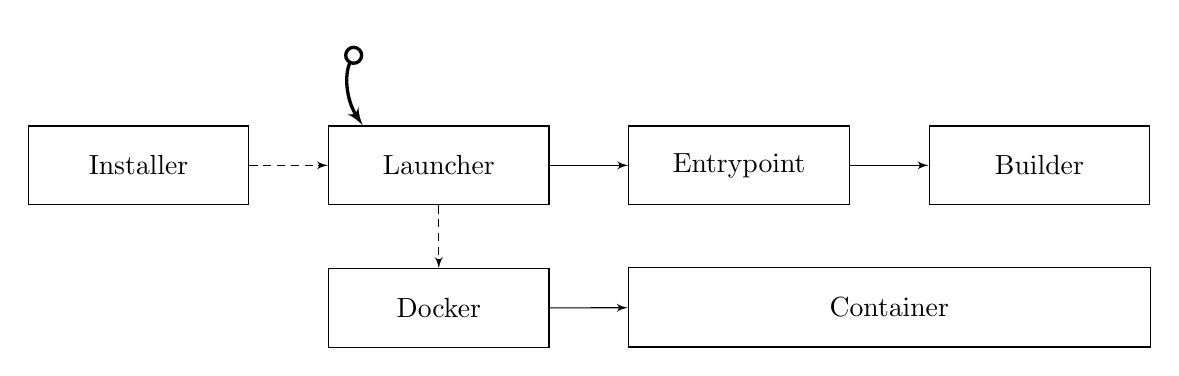
\begin{tikzpicture}[>=latex']
    \tikzset{block/.style={
      draw,
      rectangle,
      align=center,
      minimum width=2.8cm,
      minimum height=1cm
    }};

    \node [block] (installer) {Installer};
    \node [block, right=1cm of installer] (launcher) {Launcher};
    \node [block, right=1cm of launcher] (entrypoint) {Entrypoint};
    \node [block, right=1cm of entrypoint] (builder) {Builder};
    \node [block, below=0.8cm of launcher] (docker) {Docker};

    \node [
      block,
      inner sep=0pt,
      yshift=-1.8cm,
      minimum height=0.6cm,
      fit={(entrypoint) (builder)},
      label=center:Container] (container) {};

    \node [above left=1cm and -0.5cm of launcher] (start) {};

    \path[draw,->] (launcher) edge (entrypoint)
      (entrypoint) edge (builder)
      (docker) edge (container);

    \path[densely dashed,->] (installer) edge (launcher)
      (launcher) edge (docker);

    \path[draw,o->,very thick] (start) edge[bend right] (launcher);
  \end{tikzpicture}
  \caption{Execution sequence of build pipeline components.}
\end{figure}

\paragraph{Installation.} The recommended way to install the \acrshort{cli} tool is by downloading a \lstinline|bash| script and piping it to the shell. This is a pattern known as ``curl pipe sh'', and while common because of its simplicity, there are some security implications which are discussed in section~\ref{sec:limitations}. A Content Delivery Network, \emph{Cloudflare}, is used to ensure the installer script is exclusively served via \acrshort{http} over \acrshort{tls}.

\begin{lstlisting}[
  label={lst:curlpipesh},
  caption={CLI tool installation command}
]
curl https://get.beamup.io/install | /bin/sh
\end{lstlisting}

When the installer detects it is being executed inside an interactive terminal session, it pauses for a few seconds to give the user a chance to abort installation. Next, the installer clones the \acrshort{cli} repository to the \lstinline|~/.beamup| folder of the current user's home directory. Note that cloning a repository keeps file permissions intact, including the executable bits that are set on the main \acrshort{cli} launcher script. At no point are super user permissions needed, consequently the installer first attempts to create a symbolic link to the \acrshort{cli} launcher, and optionally falls back to displaying instructions on how to add the just-installed tool to the executable path. Finally, to make sure that the installation was successful, the launcher is invoked for a self-test. Because the \acrshort{cli} tool is little more than a local clone of a remote repository, distributing and installing updates to the tool itself becomes as trivial as pulling changes from the remote. A convenience wrapper is provided.

\paragraph{Transparent container invocation.} The main point of entry to the \acrshort{cli} build tool the launcher \lstinline|bash| script. It is the starting point for all invocations and its responsibility is to pass the given arguments to the \emph{container entrypoint}, either by starting a new container, or directly. Many \acrshort{ci} platforms confine the whole build process to a container that has already been set up and started, allowing only limited configuration of the container's parameters. Since it is not always possible to start a clean container, the tool must be able to either operate inside an already-running \acrshort{ci} container, or transparently start a new container and pass control inside.

First, the launcher  attempts to detect where it is being called from by parsing the \emph{\acrfull{cgroup}} file. While detection in this way is widespread, it is not recommended, since it relies on an implementation detail of the container runtime. However, work to add container introspection capabilities is ongoing\footnote{\url{https://github.com/moby/moby/pull/26331}}. To provide a temporary solution until an interface is finalized and widely deployed, the tool checks for artifacts of common container runtime implementations in the \acrshort{cgroup} file: \emph{Docker}, \emph{\acrfull{lxc}}, and \emph{\acrfull{aws} \acrfull{ecs}}. If the tool is being run inside a container, execution is simply passed to the \emph{container entrypoint} along with all arguments under the assumption that the container's environment is sufficiently correct, i.e.~has the correct version of Erlang/OTP installed.


\paragraph{Determining the base image.} When the launcher determines that it is able to start a container to run the build in, i.e.~the tool is being invoked inside a \acrshort{vm} or on bare metal, it needs to consider the following two attributes to determine which image to instantiate a container from:
\begin{enumerate*}[label=(\roman*)]
  \item The requested version of Erlang/OTP, read from an environment variable, and
  \item the host's machine architecture.
\end{enumerate*}

Concerning the machine architecture, official builds of Erlang/OTP for various architectures are provided on the \emph{Docker Hub}. Such images are available under the namespace of the respective architecture identifiers as used by the \emph{Go} programming language. A challenge lies in reliably normalizing the machine architecture as reported by \lstinline|uname -m|. Note that since version \emph{17.06 Docker} implicitly pulls images for the correct architecture. However, because the tool is designed to support \emph{Docker} down to version \emph{1.12}, the launcher has to manually determine the architecture and map it to an image namespace identifier using the following normalization table.

\begin{table}[h]
  \setlength{\tabcolsep}{10pt}
  \centering
  \begin{tabular}{ r l }
    Output of \lstinline|uname -m| & Identifier \\
    \hline
    \lstinline|arm arm32 armv7 armv7l armhfp| & \lstinline|arm32v7| \\
    \lstinline|arm64 armv8 armv8b armv8l aarch64 aarch64_be| & \lstinline|arm64v8| \\
    \lstinline|i386 i686 i686-64 i686-AT386| & \lstinline|i386| \\
    \lstinline|s390x s390| & \lstinline|s390x| \\
    \lstinline|ppc ppc64 ppcle ppc64le| & \lstinline|ppc64le| \\
    \emph{other} & \lstinline|amd64| \\
  \end{tabular}
  \caption{Mapping between reported machine architecture and image identifier.}
\end{table}

Note that support for other \acrshort{beam} languages such as Elixir is handled within the \emph{container entrypoint}, and it is sufficient to pull an image containing just the Erlang/OTP runtime at this point. Additionally, there are currently no official images of Elixir available for all machine architectures supported by the Erlang/OTP images.


\paragraph{Project mount.} Clearly, the build tool needs access to the directory containing the Erlang/OTP project to be built. The launcher is meant to be invoked inside that directory, and derives the project's name from the name of the current working directory. Note that the build tools must be able to freely modify various configuration files of the project, e.g.~overwrite version numbers, add dependencies and output artifacts. However, the tools must not permanently alter any files of the original project folder on the host as doing so may interfere with other parts of the build pipeline.

Ideally, the project folder would be mounted as a layered \acrfull{cow} filesystem where the tools may modify any files in a writable upper layer that is overlaid above the original read-only project folder. However, creating \emph{overlay filesystem} mounts inside a container requires elevated privileges of the container as well as additional configuration on the host. Therefore, \acrshort{cow} filesytem mounts are out on \acrshort{ci} platforms. Another way to implement rollback capabilities would be to exploit a \acrfull{scm} system such as Git to track changes made to the project folder. This approach is not optimal either; as \begin{enumerate*}[label=(\roman*)]
  \item it would require to strip existing Git metadata from the project; and
  \item Git is not recommended for tracking changes to binary files such as compressed release artifacts.
\end{enumerate*}

Therefore the naïve solution chosen for this tool is to first mount the project folder as a read-only volume into the container, and then create temporary working copies on which the tools operate without restriction. The original project folder on the host cannot be edited by any process inside the container. Note that if the tool is started inside an already-running container, said restriction of read-only volumes does not apply and the tool must take care to never modify the original location by first creating a copy to a temporary location.


\paragraph{Cache mount.} Minimizing build run time is crucial for a pleasant \acrlong{ci} workflow. Many \acrshort{ci} platforms offer a way to cache the contents of certain folders between build runs. A number of cache folders of the container are bind-mounted to a single cache path in the host user's home directory. Combining the cache paths into one folder on the host makes it trivial to setup caching, as instead of having to configure multiple, possibly changing paths for each tool separately, it is sufficient to cache just one folder. Currently, the host cache folder combines bind mounts of the following locations inside the container:
\begin{itemize}
  \item Compiled artifacts and dependencies of the build tool itself;
  \item Dependency cache directories of the build tools \lstinline|rebar3| and \lstinline|mix|;
  \item Erlang and Elixir interactive shell history files;
  \item Precompiled, downloaded, and extracted Elixir release.
\end{itemize}
Note that if the launcher is unable to start a container, caching would have to be set up explicitly for each location.

\paragraph{Virtual RAM disk.} The run time of the build tool is bound by performance of the filesystem and storage media. Additionally, building upgrade releases causes the entire project folder to be temporarily duplicated for each previous release.
If supported by the \emph{Docker} client, the container's \lstinline|/tmp| directory is mounted as a temporary filesystem (\emph{tmpfs}) on the host's \acrshort{ram}. In case the size of the temporary file system grows beyond the available \acrshort{ram}, the host \acrshort{os} transparently falls back to consuming swap space.

\paragraph{Project scaffolding.} To quickly create basic folder structure and files for new projects in various \acrshort{beam} languages, the \acrshort{cli} provides a convenience command.

\paragraph{Environment variables.} All configuration for the tool is provided via environment variables, instead of files or interactive menus. Most \acrlong{ci} platforms provide a straightforward way to configure environment variables for the build pipeline, and many offer additional facilities to encrypt or otherwise store environment variables in a secure way. The launcher reads various environment variables and other parameters of the host, applies transformations, and passes configuration on to the \emph{container entrypoint}, again via environment variables.

Table~\ref{table:envvars} lays out how various parts of the build pipeline use environment variables to pass and transform configuration. Note that neither the architecture of the host, nor the architecture part of the image identifier are passed into the container, as the builder internally retrieves the system architecture string as reported by Erlang/OTP, which differs from the identifier used at the launcher stage.

\begin{table}[h]
  \setlength{\tabcolsep}{10pt}
  \centering
  \begin{tabularx}{\textwidth}{l X X}
    Host & Launcher & Container entrypoint \\
    \hhline{===}
    \emph{working directory} &
      passed as \lstinline|PROJECT_DIR| \newline
      either as-is or with container path of mount point &
      passed through \\
    \hline
    \lstinline|ERLANG_VERSION| &
      used to determine \newline
      image identifier &
      validated against \newline
      currently installed version \\
    \hline
    \lstinline|ELIXIR_VERSION| &
      passed through &
      used to validate and/or \newline
      install Elixir \\
    \hline
    --- &
      \lstinline|TERM| set to \lstinline|dumb| &
      passed through \\
    \hline
    --- &
      contents read from global gitignore
      file and passed on as \lstinline|GLOBAL_GITIGNORE| &
      contents written to \newline
      container's global \newline
      \emph{gitignore} file \\
    \hline
    \lstinline|STORE| & passed through & passed through \\
    \hline
    \lstinline|STORE_SECRET| & passed through & passed through \\
    \hline
    \lstinline|DEBUG| & passed through & passed through \\
  \end{tabularx}
  \caption{Transformation of environment variables between host and container.}
  \label{table:envvars}
\end{table}



\subsection{Builder}

\paragraph{Container entrypoint.} As stated above, the \acrshort{cli} may be launched inside an already-running container, or start a clean container. In any case, the \emph{container entrypoint} is a \lstinline|bash| script that is always executed inside a container. Yet it may only make minimal assumptions about its environment since the container may have been set up already with parameters beyond the launcher's control. The primary job of the container entrypoint is to compile the builder. It is also responsible for setting up the Erlang code path to include the location of the builder's compiled artifacts, and to add the directory containing the \emph{command \acrshort{escript}s} to the system's executable path. Finally, the container entrypoint script calls \lstinline|exec $@| to replace the execution of itself with the program whose name and arguments were passed through by the \acrshort{cli} launcher. Such constructs are common in container entrypoint scripts, as doing so allows to transparently invoke any executable inside the container as if the program was running on the host, while preparing the environment before passing control onwards.

\paragraph{Command escripts.} \acrlong{escript}s (\acrshort{escript}s) provide a way to transparently call Erlang code from the system's shell. Some of the tool's commands, including ``build'', ``self test'', and ``install elixir'' are implemented as \acrshort{escript}s. They act as thin wrappers for the Erlang modules that make up the builder application. Their responsibility is to read from various environment variables and to supply them as valid arguments to the builder application.

\subsection{Store}

\section{Discussion}


\subsection{Advantages}

\paragraph{Hands-off operation.} The tool is meant to be used as part of a \acrfull{ci} pipeline. Invoking a single command generates a deployable artifact from a checkout of the code base. Version identifiers are generated from commit timestamps and hashes, \acrfull{appup} are generated on a best-effort basis. Previous releases are fetched from the central release store, where the newly generated release artifact is uploaded to.

\paragraph{Installation.} The \acrshort{cli} build tool is installed with a single command that does not need superuser permissions, is not dependent on a specific package manager, and has no dependencies except \lstinline|curl|, \lstinline|bash| and Git, which can safely be assumed to exist on the system.

\paragraph{\acrshort{ci} support.} The tool has been shown to work on at least six common hosted \acrfull{ci} providers: \emph{Travis \acrshort{ci}, Codeship, Circle \acrshort{ci}, Wercker, Semaphore,} and \emph{Shippable}. Build run time and setup effort are comparable across providers.

\paragraph{Declarative.} The command to start a build is always the same, there are no flags or parameters. All settings such as authentification credentials for the store, or the version of Erlang/Elixir to use are passed to the tool via environment variables. The build process requires no interaction.

\paragraph{Single cache.}  Instead of having to configure and maintain multiple cache paths that may change in the future, the cache locations of various tools used within the build process are consolidated inside one directory.

\paragraph{Normalized environment.} The tool detects whether it is being run directly on a \acrshort{vm}, in which case it attempts to normalize the environment by starting a container. Nevertheless, the tool aims to be well-behaved with respect to its environment.

\paragraph{Read only.} The tool never modifies the original project folder. All operations happen on temporary copies, preferably on a \acrshort{ram} disk, and the only artifact produced by a build run is a single deployable tarball. The compressed release artifact is either directly uploaded to a remote store, or written to the file system as specified by an environment variable.

% --

\cleardoublepage
\subsection{Limitations}

\paragraph{Installer.}\label{sec:curlpipesh} Distributing the \acrshort{cli} tool by downloading a script and piping it to the shell, thereby immediately executing its arbitrary contents may appear to be unsafe. Yet, there is not yet a simpler solution. The \acrshort{cdn} that serves the installer script is configured to only accept connections over \acrshort{tls}, and \lstinline|curl| verifies the validity of the certificate. The installer is wrapped in a shell function to guard against executing a partially downloaded script. Besides, those concerned about the security implications can circumvent the installer by manually cloning a vetted checkout of the \acrshort{cli} repository.

\paragraph{Linux only.} Since the build process always runs inside a Linux container, the resulting release artifact only runs on Linux systems as well. Note that the \acrshort{cli} tool itself may be invoked on other \acrshort{os}es where Docker is supported, such as macOS, as the Docker client will then transparently run the container on a virtualized Linux kernel. Thus, the built release still only supports Linux.

\paragraph{Minimal customization.} The tool aims to cover only the most common default project configurations. This implies that all configuration files for the respective tools are in their standard locations, and that the project is set up like the scaffolding generated by the \lstinline|beamup new| command. Advanced features of the build tools such as build profiles or multiple releases are not supported.

\paragraph{Already-containerized pipeline.} All but one of the tested \acrshort{ci} providers run the build inside a preconfigured container, with only Travis \acrshort{ci} offering the choice between a container or a \acrshort{vm}. When the container has already been started, the launcher cannot make certain optimizations. Namely, it cannot mount a \acrshort{tmpfs} \acrshort{ram} disk, or consolidate the cache folders. The tool must also assumes that the correct version of Erlang/\acrshort{otp} is already installed.

\paragraph{High \acrshort{ram} or disk usage during build.} The project folder is duplicated multiple times during the build process, at least twice for every upgrade from a previous release. The tool attempts to keep the number of concurrently existing duplicates minimal. To avoid disk thrashing, the tool attempts to copy the project onto a \acrshort{ram} disk.

\paragraph{Store is an active component.} The builder currently supports two backends for storing built artifacts. The release tarball may either be output to the local file system, or uploaded to the store, which is a server component that must be deployed and maintained. The current feature set implies that an active store component is unnecessary, and a backend for e.g.~a simple object storage would suffice. The \acrshort{api} and implementation of the store server component is incomplete and will in the future be extended to cover additional aspects of release handling, such as deploying releases to a fleet of nodes.

\paragraph{Possibly unnecessary downloading of previous releases.} The tool currently downloads the entirety of all previous releases to generate upgrade instructions. An alternative would be to locally check out the previous commits to upgrade from, compile each previous release from the checked out code, and then to compare them to generate upgrade instructions. This work has not evaluated advantages or limitations of a local-only approach.

\paragraph{Machine architecture support.} Though untested, the tool should be able to run on various machine architectures, and produce releases runnable on the respective architectures: \lstinline|amd64|, \lstinline|arm32v7|, \lstinline|arm64v8|, \lstinline|i386|, \lstinline|ppc64le|, \lstinline|s390x|. However,  it has not been tested on any machine architectures except \lstinline|amd64| and \lstinline|arm64v8|. There is also no cross-compilation support, or support for compiling additional native dependencies as Erlang \acrfull{nif}.

\paragraph{Best-effort \acrshort{appup} generation.} The build tool trades full control over the build process for hands-off operation. In certain situations with complicated dependencies between modules, processes, or even nodes the algorithm for generating \acrfull{appup}files may produce incorrect results.

\cleardoublepage
\section{Related Work}\label{sec:related_work}

\paragraph{Knit.}\cite{davis:knit,davis:talk} Knit aims for similar usability goals; requiring just one command to generate a \acrshort{dsu}-capable release from previous packages. Knit relies on the build tool \lstinline|rebar|, which – unlike its successor \lstinline|rebar3| - includes an algorithm similar to~\cite{rebar3appup} for generating \acrshort{appup}s. Knit optionally takes metadata hints from the developer via \emph{module attributes} to guide \acrshort{appup} generation. The project appears to be no longer maintained.

\paragraph{Distillery.}

\paragraph{Edeliver.}

\paragraph{Erlang on Nix.} The package manager Nix~\cite{nix1} borrows ideas from functional programming: immutability, pure functions, referential transparency. Its artifacts are identified via cryptographic hashes of all inputs used to build them. Nix provides repeatable environments to build packages inside, similar to what containers are used for in this work, but with stronger determinism. Nix forms the base of NixOS~\cite{nixos}, a full-featured Linux distribution where the all its components are managed by Nix via symbolic links.
Work by~\cite{erlangnix} allows dependencies of Erlang/\acrshort{otp} projects to be managed via Nix, and \cite{erlangnix2}~presents a pipeline to deploy Erlang/\acrshort{otp} projects with Nix.

% --
\cleardoublepage
\section{Future Work}

\paragraph{Hands-off deployment.}


\paragraph{Update safeness.}

Add Preprocessing step for native dependencies, asset pipeline

investigate how


Measure how often automatic appup generation succeeds/fails in a real project

Statically verify update safeness properties, develop an update safety linter
Add code signing of built artifacts

Adapt to other BEAM Languages and SCM systems
Evaluate support on ARM CPU architectures.

% --
\cleardoublepage
\section{Conclusion.}

\cleardoublepage
\section{Future Work}

An an immediately adjacent task would be to design a similarly hands-off way to deploy the built artifacts. This would include bootstrapping infrastructure, performing \acrshort{dsu}, and runtime inspection.

Part of the recent surge of interest in the Erlang/\acrshort{otp} ecosystem is driven by alternative \acrshort{beam} languages, notably Elixir. While the described tool supports Elixir, it should be improved for better handling native dependencies



Similarly, configuration management.


Add code signing of built artifacts

Adapt to other BEAM Languages and SCM systems
Evaluate support on ARM CPU architectures.


investigate how

It would be interesting to collect empirical data on how often automated best-effort \acrshort{appup} generation using~\cite{rebar3appup} or other algorithms for \acrshort{dsu} succeeds or fails in a real-world project.

There is a large body of ongoing research studying update safeness properties of various languages and \acrshort{dsu} systems.

Statically verify update safeness properties, develop an update safety linter

% --
\cleardoublepage
\section{Conclusion.}

This work has shown how the Erlang/\acrshort{otp} release generation process can be automated to a degree where


\include{lists}

\bibliography{lit}
\bibliographystyle{alpha}

\end{document}
